% This file was created with tikzplotlib v0.10.1.
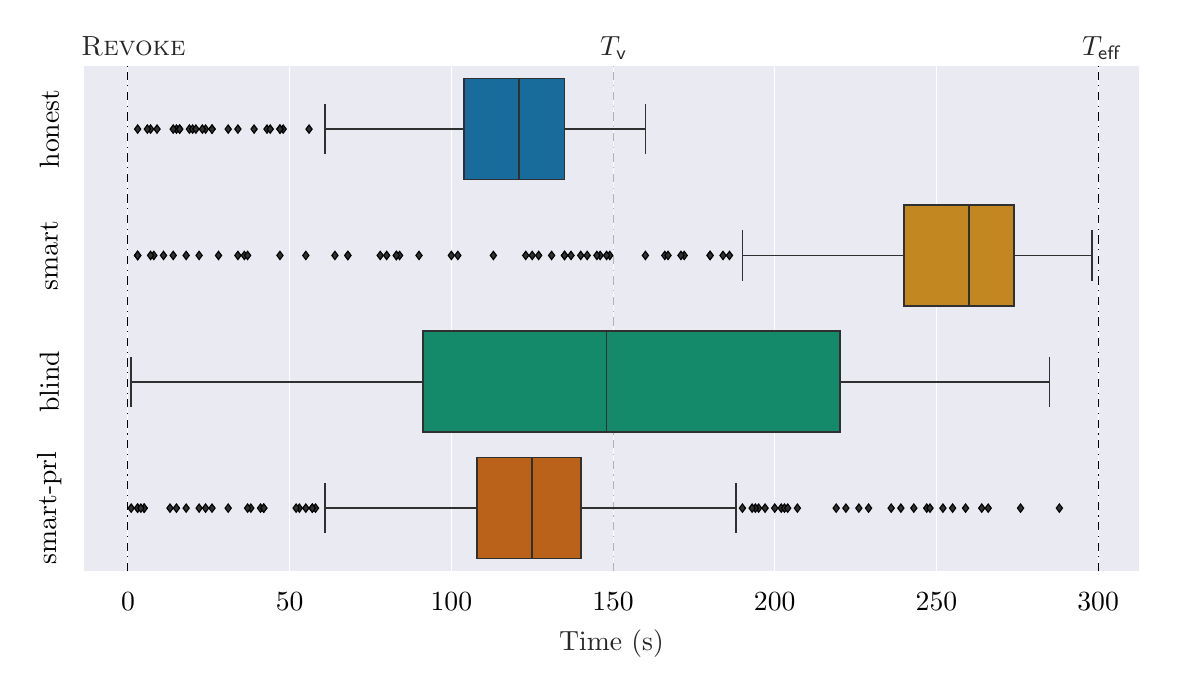
\begin{tikzpicture}

\definecolor{chocolate1869726}{RGB}{186,97,26}
\definecolor{darkgoldenrod19413532}{RGB}{194,135,32}
\definecolor{darkslategray38}{RGB}{38,38,38}
\definecolor{darkslategray48}{RGB}{48,48,48}
\definecolor{lavender234234242}{RGB}{234,234,242}
\definecolor{seagreen21138106}{RGB}{21,138,106}
\definecolor{teal23108155}{RGB}{23,108,155}

\begin{axis}[
clip=false,
axis background/.style={fill=lavender234234242},
axis line style={white},
height=8cm,
minor xtick={},
minor ytick={},
tick align=outside,
width=15cm,
x grid style={white},
xlabel=\textcolor{darkslategray38}{Time (s)},
xmajorgrids,
xmajorticks=true,
xmin=-13.85, xmax=312.85,
xtick style={color=darkslategray38,draw=none},
xtick={-50,0,50,100,150,200,250,300,350},
y dir=reverse,
y grid style={white},
ymajorticks=true,
ymin=-0.5, ymax=3.5,
ytick style={color=darkslategray38,draw=none},
ytick={0,1,2,3},
yticklabel style={rotate=90.0,anchor=center,yshift=8pt},
yticklabels={honest,smart,blind,smart-prl}
]
% START VERTICAL LINES %
\addplot [dashdotted, black]
table {%
0 3.5
0 -0.5
};
\addplot [dashdotted, gray!60]
table {%
150 3.5
150 -0.5
};
\addplot [dashdotted, black]
table {%
300 3.5
300 -0.5
};
% END VERTICAL LINES %
\path [draw=darkslategray48, fill=teal23108155, semithick]
(axis cs:104,-0.4)
--(axis cs:104,0.4)
--(axis cs:135,0.4)
--(axis cs:135,-0.4)
--(axis cs:104,-0.4)
--cycle;
\path [draw=darkslategray48, fill=darkgoldenrod19413532, semithick]
(axis cs:240,0.6)
--(axis cs:240,1.4)
--(axis cs:274,1.4)
--(axis cs:274,0.6)
--(axis cs:240,0.6)
--cycle;
\path [draw=darkslategray48, fill=seagreen21138106, semithick]
(axis cs:91.25,1.6)
--(axis cs:91.25,2.4)
--(axis cs:220.25,2.4)
--(axis cs:220.25,1.6)
--(axis cs:91.25,1.6)
--cycle;
\path [draw=darkslategray48, fill=chocolate1869726, semithick]
(axis cs:108,2.6)
--(axis cs:108,3.4)
--(axis cs:140,3.4)
--(axis cs:140,2.6)
--(axis cs:108,2.6)
--cycle;
\addplot [semithick, darkslategray48]
table {%
104 0
61 0
};
\addplot [semithick, darkslategray48]
table {%
135 0
160 0
};
\addplot [semithick, darkslategray48]
table {%
61 -0.2
61 0.2
};
\addplot [semithick, darkslategray48]
table {%
160 -0.2
160 0.2
};
\addplot [black, mark=diamond*, mark size=1.5, mark options={solid,fill=darkslategray48}, only marks]
table {%
3 0
26 0
48 0
7 0
19 0
15 0
47 0
31 0
6 0
9 0
20 0
39 0
47 0
34 0
26 0
43 0
24 0
56 0
44 0
14 0
16 0
21 0
23 0
16 0
};
\addplot [semithick, darkslategray48]
table {%
240 1
190 1
};
\addplot [semithick, darkslategray48]
table {%
274 1
298 1
};
\addplot [semithick, darkslategray48]
table {%
190 0.8
190 1.2
};
\addplot [semithick, darkslategray48]
table {%
298 0.8
298 1.2
};
\addplot [black, mark=diamond*, mark size=1.5, mark options={solid,fill=darkslategray48}, only marks]
table {%
135 1
127 1
3 1
68 1
90 1
180 1
113 1
149 1
123 1
186 1
83 1
180 1
146 1
137 1
166 1
8 1
7 1
78 1
3 1
160 1
28 1
64 1
22 1
68 1
125 1
47 1
172 1
140 1
36 1
55 1
148 1
80 1
171 1
145 1
3 1
102 1
14 1
184 1
18 1
34 1
100 1
84 1
11 1
142 1
131 1
83 1
37 1
135 1
167 1
};
\addplot [semithick, darkslategray48]
table {%
91.25 2
1 2
};
\addplot [semithick, darkslategray48]
table {%
220.25 2
285 2
};
\addplot [semithick, darkslategray48]
table {%
1 1.8
1 2.2
};
\addplot [semithick, darkslategray48]
table {%
285 1.8
285 2.2
};
\addplot [semithick, darkslategray48]
table {%
108 3
61 3
};
\addplot [semithick, darkslategray48]
table {%
140 3
188 3
};
\addplot [semithick, darkslategray48]
table {%
61 2.8
61 3.2
};
\addplot [semithick, darkslategray48]
table {%
188 2.8
188 3.2
};
\addplot [black, mark=diamond*, mark size=1.5, mark options={solid,fill=darkslategray48}, only marks]
table {%
42 3
57 3
31 3
3 3
5 3
22 3
26 3
13 3
5 3
18 3
58 3
1 3
3 3
41 3
4 3
24 3
42 3
55 3
57 3
38 3
53 3
15 3
52 3
37 3
276 3
202 3
222 3
229 3
195 3
219 3
194 3
193 3
264 3
266 3
236 3
207 3
200 3
226 3
259 3
247 3
203 3
204 3
243 3
248 3
239 3
288 3
197 3
252 3
255 3
190 3
};
\addplot [semithick, darkslategray48]
table {%
121 -0.4
121 0.4
};
\addplot [semithick, darkslategray48]
table {%
260 0.6
260 1.4
};
\addplot [semithick, darkslategray48]
table {%
148 1.6
148 2.4
};
\addplot [semithick, darkslategray48]
table {%
125 2.6
125 3.4
};
\draw (axis cs:-17.5,-0.58) node[
  scale=1,
  anchor=base west,
  text=darkslategray38,
  rotate=0.0
]{\textsc{Revoke}};
\draw[dashed] (axis cs:143,-0.58) node[
  scale=1,
  anchor=base west,
  text=darkslategray38,
  rotate=0.0
]{$T_{\mathsf{v}}$};
\draw (axis cs:292,-0.58) node[
  scale=1,
  anchor=base west,
  text=darkslategray38,
  rotate=0.0
]{$T_{\mathsf{eff}}$};
\end{axis}

\end{tikzpicture}
